% status: 0
% chapter: TBD

\title{Big Data Reference Architecture using Python Celery}


\author{Sabra Ossen}
\affiliation{%
	\institution{Indiana University}
	\streetaddress{Smith Research Center}
	\city{Bloomington} 
	\state{IN} 
	\postcode{47408}
	\country{USA}}
\email{sossen@iu.edu}

\author{Gregor von Laszewski}
\affiliation{%
  \institution{Indiana University}
  \streetaddress{Smith Research Center}
  \city{Bloomington} 
  \state{IN} 
  \postcode{47408}
  \country{USA}}
\email{laszewski@gmail.com}


% The default list of authors is too long for headers}
\renewcommand{\shortauthors}{G. v. Laszewski}


\begin{abstract}
Distributed Big Data reference architectures are of great importance and can 
be built by various tools supporting distributed tasks. With the use of Python 
Celery this project focuses on building such a distributed Big Data reference 
architecture. The main goal of the project is to identify the key requirements 
for the domain and build the components of the system. K-means is a widely 
known clustering algorithm that is used on a huge amount of data sets. 
Therefore, the use case for this project is built around executing the K-means 
algorithm. The environment is also built on three environments; local, 
distributed cloud and multi-container Docker environments.
\end{abstract}

\keywords{hid-sp18-416, Python Celery, Swagger REST services, Node JS, Spark, 
Hadoop}


\maketitle

\section{Introduction}

Today, big data is a highly available, crucial and necessary for every domain. 
Machine learning is the key methodology to analyze the big data obtained from 
various sources. With the high volume of big data, it becomes a necessity to 
have a distributed environment to handle the different components such as 
algorithm execution, storage, and summarization. 

This project aims on building a reference architecture for executing 
machine learning in a distributed environment. The architecture will be built 
upon several components such as Python 
Celery~\cite{hid-sp18-416-www-python-celery}, Swagger 
REST~\cite{hid-sp18-416-www-swagger}, Redis~\cite{hid-sp18-416-www-redis}, 
Apache Hadoop~\cite{hid-sp18-416-www-apache-hadoop}, 
Node JS~\cite{hid-sp18-416-www-nodejs} and 
Spark~\cite{hid-sp18-416-www-apache-spark}. The main components of the 
architecture are Python Celery and Swagger REST services. Python Celery allows 
user-responsive long-running tasks to run in the background using distributed 
task queues. 

The first phase will focus on implementing the architecture in a local 
environment and the second phase will focus on implementing it in a cloud 
environment. Amazon Elastic Compute Cloud (EC2) 
instances~\cite{hid-sp18-416-www-amazon-ec2} and 
Amazon Elastic File System (EFS)~\cite{hid-sp18-416-www-amazon-efs} will be 
used to build the distributed cloud environment. The third 
phase focuses on implementing a multi-container Docker environment for the 
distributed architecture using Docker~\cite{hid-sp18-416-www-docker} and 
Docker Compose~\cite{hid-sp18-416-www-docker-compose}. Two `Clustering' based 
datasets from the UCI Machine Learning 
repository~\cite{hid-sp18-416-www-uci-ml-repository} will be used for 
evaluation of the distributed architecture. 

The project goals are listed as follows.
\begin{enumerate}
	\item Create a Node JS Server exposing the set of functions to upload 
	to (input files) and download from (predictions and model files) in a 
	Hadoop Distributed File System (HDFS)~\cite{hid-sp18-416-www-ibm-hdfs}
	\item Execute machine learning function (K-means example) using Apache 
	Spark~\cite{hid-sp18-416-www-apache-spark}.
	\item Expose the tasks supported by the distributed Python 
	celery~\cite{hid-sp18-416-www-python-celery} workers through a Swagger REST 
	service~\cite{hid-sp18-416-www-swagger}
	\item Build the reference architecture in the local, cloud and docker 
	environments.
	\item Provide a thorough guide on building distributed Big Data analysis 
	environments.	
\end{enumerate}

\section{Technology Usage}

This section focuses on providing an overview of the many tools used in this 
project. The key tool supporting the distributed architecture is Python 
Celery~\cite{hid-sp18-416-www-python-celery} which is an asynchronous task 
queue based on distributed message passing. Node 
JS~\cite{hid-sp18-416-www-nodejs} and Swagger 
Codegen~\cite{hid-sp18-416-www-swagger-codegen} have also been used to build 
REST services exposing the file system and celery workers. Further explanation 
on tools and technologies used for building different architectures on 
different platforms is also given.

\subsection{Python Celery}

Celery is an asynchronous task queue which is based upon distributed message 
passing and uses RabbitMQ or Redis as the communication system. The smallest 
unit of execution in Python Celery is a task, which can be used to execute 
either long running or quick tasks. Celery also provides the flexibility to 
execute tasks synchronously and 
asynchronously~\cite{hid-sp18-416-www-python-celery}. Celery 
can be understood as a tool that encompasses many communication systems, 
abstractions, scheduling and real time operation handling capabilities. Celery 
is a easy to use, highly configurable, flexible and fast tool that can be used 
to handle a very large amount of tasks of varying 
nature~\cite{hid-sp18-416-www-vinta-celery-blog}.

\subsection{Node JS}

Node JS is a widely used platform supporting server side JavaScript execution. 
Node JS greatly simplifies the development and maintenance of web applications 
and has an event driven architecture. This architecture design 
provides high scalability, high throughput and support for real time 
applications~\cite{hid-sp18-416-www-nodejs-wikipedia}. Node JS is most popular 
to create single page web and IOT applications, APIs and mobile 
backends~\cite{hid-sp18-416-www-nodejs-blog}. 

\subsection{Swagger Codegen}

Swagger Codegen is an open source tool that provides ease of development for 
REST API developers by means of creating server stubs and client SDKs using 
the given OPENAPI specification. It can be categorized as a automatic API code 
generation tool. This allows developers to focus more on the API 
specification and not the service generation. Swagger Codegen also has the 
capability to generate client SDKs in many different languages including 
Python~\cite{hid-sp18-416-www-swagger-codegen}. This is a key point to use 
Swagger Codegen generated REST services to expose the tasks of the Python 
Celery workers. 

\subsection{Hadoop}

Apache Hadoop is an open source platform that supports processing very large 
data sets. The complete Hadoop eco system is targeted towards distributing the 
Big Data in the HDFS and then deploying the application or solver in each of 
the nodes in the cluster. Hadoop targets to achieve batch processing with the 
use of the MapReduce programming model and the 
HDFS~\cite{hid-sp18-416-www-apache-hadoop}. The main goal of Hadoop is to 
provide scalability, fault tolerance, flexibility and performance for batch 
processing applications. Due to the support for structured and unstructured 
data Hadoop allows organizations to quickly leverage large datasets and 
perform analysis on them~\cite{hid-sp18-416-www-hadoop-hortonworks-blog}.

\subsection{Spark}

Apache Spark is an in-memory data processing engine that is based on a 
resilient distributed dataset (RDD) architecture. Spark requires cluster 
management and a distributed file system in order to function. For a 
distributed architecture, Spark is capable of interfacing with HDFS and Hadoop 
Yarn~\cite{hid-sp18-416-www-spark-wikipedia}. Spark contains a distributed 
core engine which is responsible for execution of tasks and libraries which 
provide many different user APIs from different languages and streaming 
support. Spark also has a machine learning library called `MLlib' with a wide 
variety of machine learning algorithms used in the data science 
domain~\cite{hid-sp18-416-www-spark-hortonworks-blog}.

\subsection{Amazon EC2}

Amazons' Elastic Compute Cloud (EC2) is the most famous Infrastructure as a 
Service now. Amazon EC2 provides users the pay only for the computing 
resources they consume. This provides great flexibility and is economically 
attractive to the user. With autoscaling, EC2 also provides reliability for 
the user applications. Amongst other benefits are high end security and full 
integration for other Amazon services such as Amazon 
EFS~\cite{hid-sp18-416-www-amazon-ec2}. 

\subsection{Amazon EFS}

Amazons' Elastic File System (EFS) is a scalable file system storage provided 
by Amazon. This easily integrates with existing Amazon EC2 instances and can 
be purchased only as much as it is used. EFS supports high availability and 
scalability in its shared file system. The main attraction points for Amazon 
EFS is its simplicity and integration with either on premise or cloud 
instances. There are several uses cases such as web service hosting, content 
management and Big Data analytics for Amazon 
EFS~\cite{hid-sp18-416-www-amazon-efs}. 

\subsection{Docker Compose}

Docker Compose is a tool that is used to create multi-container Docker 
applications. Docker compose provides the capability to define and run 
multiple Docker containers with ease. It also provides easy integration of 
volumes and networking between multiple docker containers. With YAML as the 
configuration file to define the multiple services Docker Compose only focuses 
on the build, start and stop of the multiple containers at the same time. 
Individual operations on each Docker image or container is irrelevant to 
Docker Compose and it only focuses on the orchestration of the environment as 
a whole~\cite{hid-sp18-416-www-docker-compose-blog}. 
	
\subsection{Versions of the Technologies Used}

Table~\ref{tbl:technologyversions} displays the versions used for each 
technology when creating the Reference Architecture. Please note that you have 
to use the Apache Spark version which is built using the Hadoop version in 
your Hadoop deployment. Also make sure to use the pyspark, py4j versions which 
are compatible with your Apache Spark version. 

\begin{table}[htbp]
	\centering
	\caption{Versions of Technologies Used}\label{tbl:technologyversions}
	\begin{tabular}{*{2}{c}}
		\toprule
		Technology & Version \\
		\midrule
		Python & 3.6   \\
		Redis & 2.10.6  \\
		Celery & 4.1.0 \\
		hdfs (HDFS CLI) & 2.1.0 \\
		py4j & 0.10.6 \\
		numpy & 1.14.2  \\
		scipy & 0.18.1  \\
		pandas & 0.19.2  \\
		pyspark & 2.3.0   \\
		java & Oracle java 8 \\
		Apache Spark & 2.3.0 \\
		Hadoop Version used & 2.7 \\
		in Apache Spark build & \\
		Hadoop & 2.7 \\
		Swagger codegen & 2.3.1   \\
		Node JS & 9.11 \\
		Docker & CE 18.03  \\
		Docker Compose & 1.8.0  \\
		\bottomrule
	\end{tabular}
\end{table}

\section{Project Procedure}

This section focuses on providing guidance for building the distributed 
reference architecture for big data problems. The first subsection which is on 
building the environment is further divided into three sections each 
explaining the specific environments used, procedures and problems faced in 
that specific environment. The second subsection focuses on defining the 
format of the data that needs to be given to the service.   

\subsection{Building the Environment}

This subsection focuses on describing the architecture and functionality of 
the system. The architecture is built on three different types of 
environments; local, Amazon EC2 (cloud) and multi-container Docker 
environments. Further explanation on each of the environments will be given 
below.

\subsubsection{Local Environment}
\label{subsubsec:localenv}

Figure~\ref{fig:localarchitecture} shows the Big Data reference architecture 
built in the local environment having the following hardware specification.

\begin{description}
	\item[Sony Vaio Laptop] 4 hardware cores, 2 threads per core, Intel Core 
	i7-2670QM processor (up to 2.2 GHz) with 8 GB DDR4 RAM, 500 GB SSD hard 
	drive and Nvidia GeForce GT 540M 1GB VGA.
\end{description}

\begin{figure}[htbp] 
	\centering
	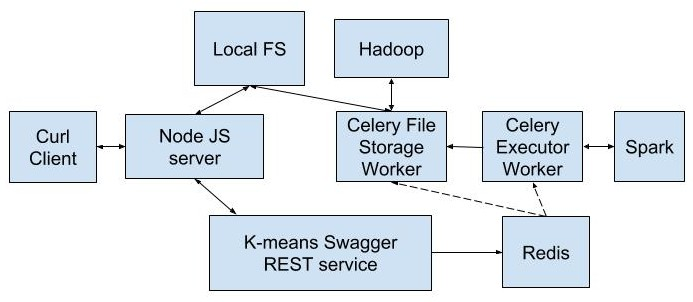
\includegraphics[width=\columnwidth]{images/localarchitecture.jpg}
	\caption{Local Architecture Environment}
\label{fig:localarchitecture} 
\end{figure}

Following is the brief overview of the functionality and architecture 
of the system. The Node JS server will be used to interact with the local file 
system which will be used to store the input data, model and prediction data. 
Following are the APIs exposed by the Node JS server.

\begin{description}
	\item[Save input file] Given the input data file in a specific format which 
	will be discussed in~\ref{sec:dataformat} save the file in the local file 
	system.
	\item[Execute KMeans] Execute K-means for the given input data set.
	\item[Get Kmeans Model] After executing K-means retrieve the model or 
	cluster centers.
	\item[Get Predictions] After executing K-means retrieve the predictions for 
	each data point.
\end{description}

A curl client can be used to invoke the functionalities which are exposed by 
the Node JS server. Next the Celery file storage and executor workers are both 
listening to the Redis Server to which the Kmeans Swagger REST service 
publishes messages after it is being invoked by the Node JS server. Both of 
the workers each listen to a specific queue and once a request (for a specific 
task) arrives in their queues they are listening to they execute the tasks. 
The file storage worker is responsible for moving the files to and from HDFS 
and the local file system. The executor worker is responsible for executing 
K-means using Spark.

\subsubsection{Distributed Cloud Environment}
\label{subsubsec:distributedcloud}

Figure~\ref{fig:distributedec2architecture} shows the Big Data reference 
architecture built in the Amazon EC2 cluster with the use of the following 
different EC2 node types.

\begin{description}
	\item[t2.small] 2 nodes for Node JS server and Hadoop installation
	\item[t2.medium] 1 node for the installation of K-means Swagger REST 
	service, celery workers, redis and spark installations
\end{description}

The hardware specification for each of the instance types is shown 
below~\cite{hid-sp18-416-www-amazon-instance-types}.

\begin{description}
	\item[t2.micro node] 1 vCPU, Intel Xeon Family Processor (up to 3.3 GHz) 
	with 1 GB RAM, Intel AVX and Intel Turbo support
	\item[t2.medium node] 2 vCPU, Intel Xeon Family Processor (up to 3.3 GHz) 
	with 4 GB RAM, Intel AVX and Intel Turbo support
\end{description}

\begin{figure}[htbp] 
	\centering
	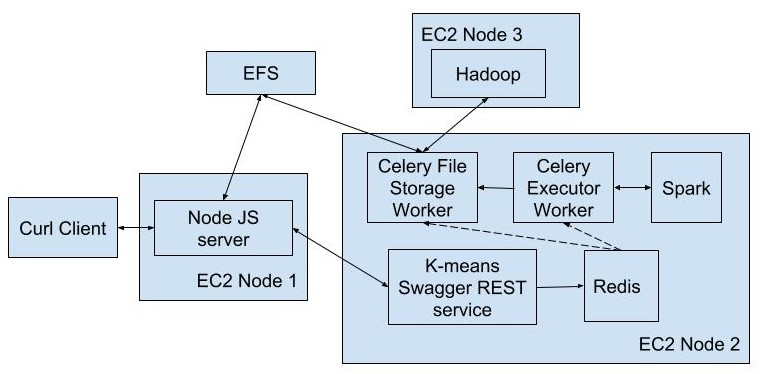
\includegraphics[width=\columnwidth]{images/distributedec2architecture.jpg}
	\caption{Distributed Architecture in EC2 Cluster}
\label{fig:distributedec2architecture} 
\end{figure}

The following paragraphs will explain how the communication between 
each of the components in the distributed architecture happens. It should be 
noted that requests are represented in black arrows and responses are 
displayed in red dashed arrows. The black dashed arrows represent that the 
Celery workers listen to the Redis servers. It should also be noted that the 
communication between from the Node JS server to the K-means Swagger REST 
service and the communication between the K-means Swagger REST service and 
Celery Workers are asynchronous.

\paragraph{Save Input Data File}

Figure~\ref{fig:uploadipfiledistributed} shows the order of request and 
response flow within the distributed architecture. 

\begin{figure}[htbp] 
	\centering
	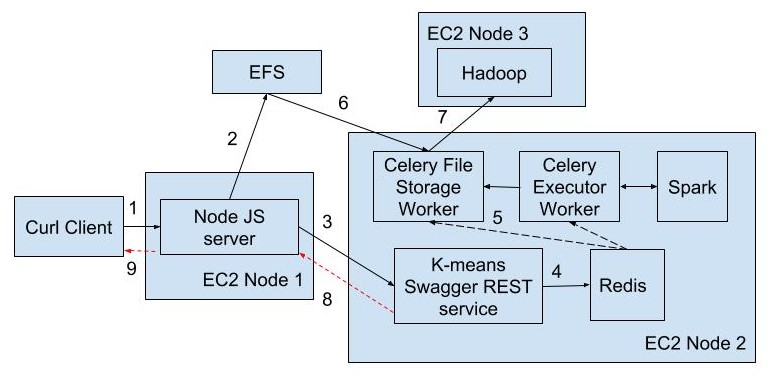
\includegraphics[width=\columnwidth]{images/ec2uploadipfile.jpg}
	\caption{Upload Input File Request/Response Flow in Distributed 
	Architecture}
\label{fig:uploadipfiledistributed} 
\end{figure}

\paragraph{Execute K-means Function}

Figure~\ref{fig:executekmeansdistributed} shows the order of request and 
response flow within the distributed architecture for executing the K-means 
algorithm.

\begin{figure}[htbp] 
	\centering
	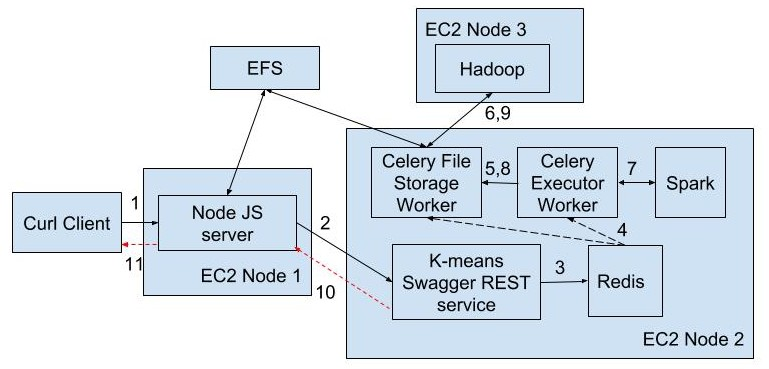
\includegraphics[width=\columnwidth]{images/ec2executekmeans.jpg}
	\caption{Execute K-means Function Request/Response Flow in Distributed 
	Architecture}
\label{fig:executekmeansdistributed} 
\end{figure}

\paragraph{Retrieve Model File}

Figure~\ref{fig:retrievemodelfiledistributed} shows the order of request and 
response flow within the distributed architecture for retrieving the K-means 
model. The same flow can be seen when retrieving the predictions for the input 
data.

\begin{figure}[htbp] 
	\centering
	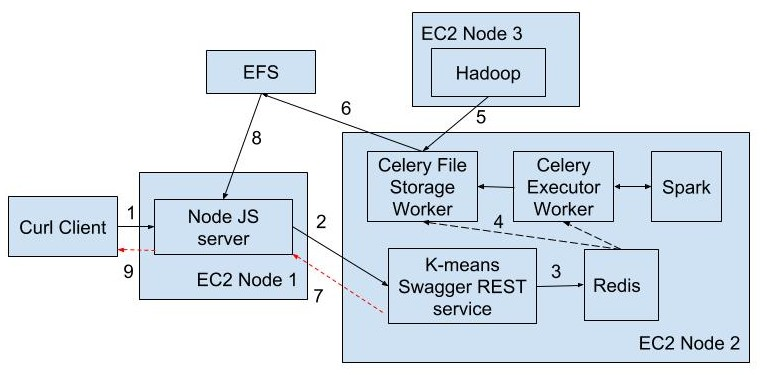
\includegraphics[width=\columnwidth]{images/ec2getkmeansmodel.jpg}
	\caption{Retrieve Model File Request/Response Flow in Distributed 
	Architecture}
\label{fig:retrievemodelfiledistributed} 
\end{figure}

\subsubsection{Multi Docker Container Environment}

Figure~\ref{fig:multicontainerdocker} shows the components of the Big Data 
reference architecture in multiple docker containers. Each of the Hadoop, Node 
JS server, K-means Swagger REST service, Redis server, Celery file storage 
worker are in single containers while the Celery executor worker and Spark 
installation are in a single container. With the help of Docker Compose we can 
easily define the network through which each of the containers will 
communicate with each other and easily mount the same file system for the file 
storage worker and Node JS server. 

\begin{figure}[htbp] 
	\centering
	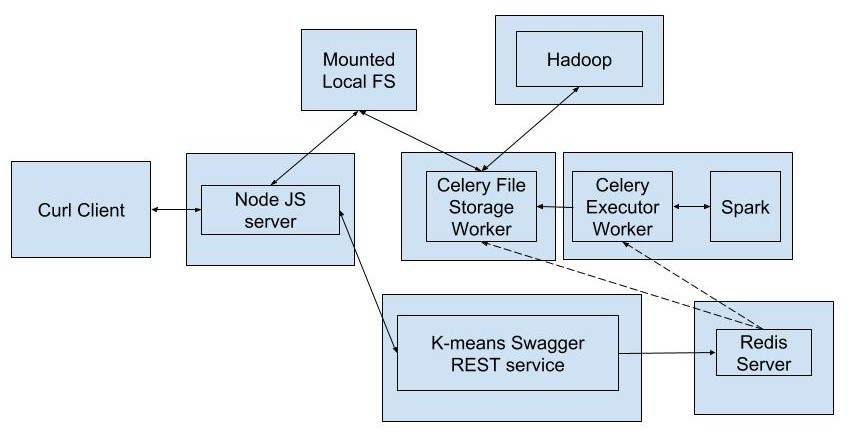
\includegraphics[width=\columnwidth]{images/dockerarchitecture.jpg}
	\caption{Multi-Container Docker Architecture}
\label{fig:multicontainerdocker} 
\end{figure}

\subsection{Data Format}
\label{sec:dataformat}

K-means can only be executed on numeric data. Therefore a pre-defined format 
in which the data should be given to the system is described here. 
Table~\ref{tab:dataformatexample} shows the format of the data for the first 
three rows. The first column should contain the id by which we can identify 
the row. Consequently the other columns should contain the numeric feature 
data, make sure to only enter numeric data as the values will be cast to a 
`double'. The column names should be given as the first row of the dataset. 
This input data file may contain `na' values as the Celery executor worker 
performs removal of `na' values from the dataset. Please note that the column 
names should only contain `\_' as a separator.

\begin{table}[htbp]
\caption{Iris Data Set Representation 
	Example~\cite{hid-sp18-416-www-iris-dataset}}\label{tab:dataformatexample}
	\centering
	\begin{tabular}{*{5}{c}}
		\toprule
		id   & sepal\_length   & sepal\_width  & petal\_length   & 
		petal\_width   \\
		\midrule
		row0 & 5.1 & 3.5 & 1.4 & 0.2 \\
		row1 & 4.9 & 3   & 1.4 & 0.2 \\
		row2 & 4.7 & 3.2 & 1.3 & 0.2 \\
		\bottomrule
	\end{tabular}
\end{table}

Figure~\ref{fig:irisinputdata} shows the classification for each of the 
flower types `Iris Setosa', `Iris Versicolor' and `Iris Virginica' against the 
Sepal\_Length and Sepal\_Width.

\begin{figure}[htbp] 
	\centering
	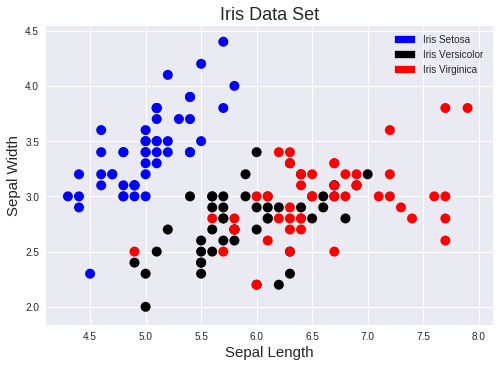
\includegraphics[width=0.8\columnwidth]{images/irisinputdata.png}
	\caption{Iris Input Data Set Classification}
\label{fig:irisinputdata} 
\end{figure}

\subsection{Expected Results}

The user can execute the K-means function with input data in the format 
described in Section~\ref{sec:dataformat}. The following files will be 
generated as output from the system.

\begin{description}
	\item[Model File] containing the cluster centers will be saved in HDFS.
	\item[Predictions File] for the input data is 
	generated such that each input data point is assigned to the cluster to 
	which it is nearest is also saved in HDFS.
\end{description}

Figure~\ref{fig:irispredictions} shows the predictions obtained after 
executing the K-means function. When comparing the predictions obtained from 
the system after executing K-means and the original classifications it can be 
seen that the system produces accurate results.

\begin{figure}[htbp] 
	\centering
	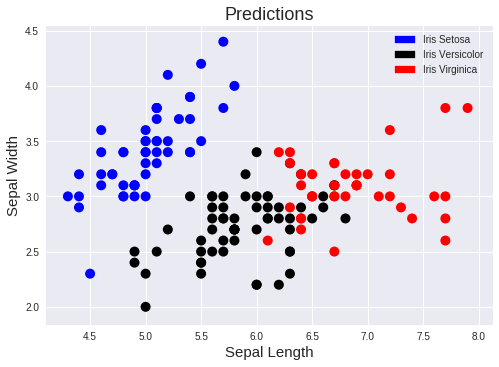
\includegraphics[width=0.8\columnwidth]{images/irispredictions.png}
	\caption{Predictions for Iris Data Set}
\label{fig:irispredictions} 
\end{figure}

\section{Results}

This section presents the time breakdown results obtained when executing the 
system in local and cloud environments. The specification of the local and 
cloud environments can be found in Section~\ref{subsubsec:localenv} 
and~\ref{subsubsec:distributedcloud}.

\subsection{Time Breakdown According to Task}

\begin{table}[htbp]
	\centering
	\caption{Task Time Breakdown}\label{tbl:tasktimebreakdown}
	\begin{tabular}{*{3}{c}}
		\toprule
		Task                                     & Time in Local & Time in EC2 
		\\
		   & Environment (s) & Environment (s) \\
		\midrule
		Upload Input File  
		&                               &                             \\
		(Total)  
		&                               &                             \\ 
		\midrule
		Upload Input File  
		&                               &                             \\
		(Request Reaching)  
		&                               &                             \\
		\midrule
		Upload Input File    
		&                               &                             \\
		(Worker Processing)    
		&                               &                             \\
		\midrule
		Executing K-means    
		&                               &                             \\
		(Total)    
		&                               &                             \\
		\midrule
		Executing K-means    
		&                               &                             \\
		(Worker Processing)    
		&                               &                             \\
		\midrule
		Retrieve Model        
		&                               &                             \\
		(Total)        
		&                               &                             \\
		\midrule
		Retrieve Model      
		&                               &                             \\
		(Request Reaching)      
		&                               &                             \\
		\midrule
		Retrieve Model       
		&                               &                             \\
		(Worker Processing)       
		&                               &                             \\
		\midrule
		Retrieve Predictions  
		&                               &                             \\
		(Total)  
		&                               &                             \\
		\midrule
		Retrieve Predictions  
		&                               &                             \\
		(Request Reaching)  
		&                               &                             \\
		\midrule
		Retrieve Predictions
		&                               &                             \\
		(Worker Processing) 
		&                               &                             \\
		\bottomrule
	\end{tabular}
\end{table}


\subsection{Time Breakdown According to Number of Clusters}

\begin{table}[htbp]
	\centering
	\caption{Time Breakdown Based on Number of 
	Clusters}\label{tbl:clustertimebreakdown}
	\begin{tabular}{*{3}{c}}
		\toprule
		Number of & Total Time in Local & Total Time in EC2 \\
		Clusters & Environment (s) & Environment (s) \\
		\midrule
		10  &          &         \\ \midrule
		20  &          &         \\ \midrule
		30  &          &         \\ \midrule
		40  &          &         \\ \midrule
		50  &          &         \\ \midrule
		60  &          &         \\ \midrule
		70  &          &         \\ \midrule
		80  &          &         \\ \midrule
		90  &          &         \\ \midrule
		100 &          &         \\ \midrule
		125 &          &         \\ \midrule
		150  &          &         \\
		\bottomrule
	\end{tabular}
\end{table}

\subsection{Time Breakdown for Different Data Sizes}

\begin{table}[htbp]
	\centering
	\caption{Time Breakdown for Different Data 
	Sizes}\label{tbl:datasizestimebreakdown}
	\begin{tabular}{*{3}{c}}
		\toprule
		Data Size & Total Time in Local & Total Time in EC2 \\
		& Environment (s) & Environment (s) \\
		\midrule
		10  &          &         \\ \midrule
		20  &          &         \\ \midrule
		30  &          &         \\ \midrule
		40  &          &         \\ \midrule
		50  &          &         \\ \midrule
		60  &          &         \\ \midrule
		70  &          &         \\
		\bottomrule
	\end{tabular}
\end{table}

\section{Conclusion}

\section{Future Work}

\begin{acks}

  The authors would like to thank Dr.~Gregor~von~Laszewski for his
  support and suggestions to write this paper.

\end{acks}

\bibliographystyle{ACM-Reference-Format}
\bibliography{report} 

